\documentclass[12pt,oneside]{book}
%\usepackage[utf8]{inputenc}


\usepackage{amssymb}
\usepackage[french,english]{babel}

\usepackage{setspace}
\usepackage{amstext}
% \theoremstyle{plain}\documentclass[10pt]{•}

\RequirePackage[colorlinks,citecolor=blue,urlcolor=blue,backref=page]{hyperref}
%\usepackage{enumerate}

\usepackage{latexsym}
\usepackage{dirtytalk}
\usepackage{amsfonts}
\usepackage{amsmath}
\usepackage{amsthm}
\usepackage{algorithm2e}
\usepackage{algpseudocode}
\usepackage{epsfig,listings}
\usepackage{enumitem}
%\usepackage[latin1]{inputenc}
\usepackage{graphicx,graphics}
\usepackage{tikz}
\usepackage{tkz-graph}
%\usepackage{epsf}
\usepackage{makeidx}
\usepackage{amsmath,amsthm,array,multicol,verbatim,mathrsfs}
%\usepackage{version}
%\usepackage{times}
%\usepackage{eucal}
\usepackage{hyperref}
%\usepackage[final]{pdfpages}
%\usepackage{datetime2}

\usepackage{fancyhdr}
\usepackage{mathtools}

\usepackage[T1]{fontenc}
\usepackage{cmbright}
%\newcommand\mesheadings[1]{\textbf{#1}}
%\FormatHeadingsWith{\mesheadings}
%\setlength{\HeadRuleWidth}{0.4pt}

\marginparwidth 1in

\newtheorem*{thm*}{Theorem}
\newtheorem{thm}{Theorem}[section]
\newtheorem{claim}[thm]{Claim}
\newtheorem{cor}[thm]{Corollary}
\newtheorem{lem}[thm]{Lemma}
\newtheorem{prop}[thm]{Proposition}
\newtheorem{rem}[thm]{\bf Remark}
\newtheorem{defn}[thm]{\bf Definition}
\newtheorem{ex}[thm]{\bf Example}
\newtheorem{exe}[thm]{\bf Exercise}
\newtheorem{exe*}[thm]{\bf Exercise*}
\newtheorem{remark}{Remark}[section]
\newtheorem{exeA}[remark]{\bf Exercise(A)}
\newtheorem{question}[thm]{\bf Question}
\newtheorem{fact}[thm]{\bf Fact}

\title{Basic Graph Theory}
\author{Hrishik Koley, Bikram Halder}
\date{}

\begin{document}

\maketitle

\tableofcontents
\clearpage



\setcounter{chapter}{-1}

\mainmatter

\chapter{Introduction}
\label{c:introduction}
These notes have been prepared to serve as a basic introduction to graph theory, which is a major prerequisite for the Winter Reading Project (WRP) on Random Graphs. These notes serve as a good enough introduction to graph theory, but are in no way, an alternative to books written on graph theory. We have covered very topics, especially, only those that are absolutely required for the WRP. To learn the topic in much more depth and breadth, you can refer to \textit{"Introduction to Graph Theory"} by \textit{Douglas B. West}, \textit{"Graphs and Matrices"} by \textit{R.B. Bapat} and to \href{https://www2.math.ethz.ch/education/bachelor/lectures/fs2016/math/graph_theory/graph_theory_notes.pdf}{\textit{Benny Sudakov}'s notes}. 

I have added some simple graph theory questions in Chapter \ref{c:Exercises}, which you can try out to strengthen your concepts. Furthermore, in Chapter \ref{c:Challenge}, I have listed some open problems, so try them at your own risk.
\chapter{Basic Definitions}
Some notation : $[n] = \{1,\ldots,n\}$, $V \times V$ the usual set product, $\binom{V}{2}$ denote unordered pairs of distinct elements in $V$. 
%
\begin{defn}(\index{Graph}Graph).  
A (simple) graph $G$ consists of a finite vertex set $V := V(G)$ and an edge set $E := E(G) \subset \binom{V}{2}.$  
\end{defn}
Before diving deeper, we first define some classes of graphs.
\begin{enumerate}
    \item \textbf{Undirected graph}: When an edge $e$ in a graph is represented by $(x,y)$ and $(x,y)=(y,x)$, then such a graph is called an undirected graph.
    \begin{figure}[hbt!]
        \centering
	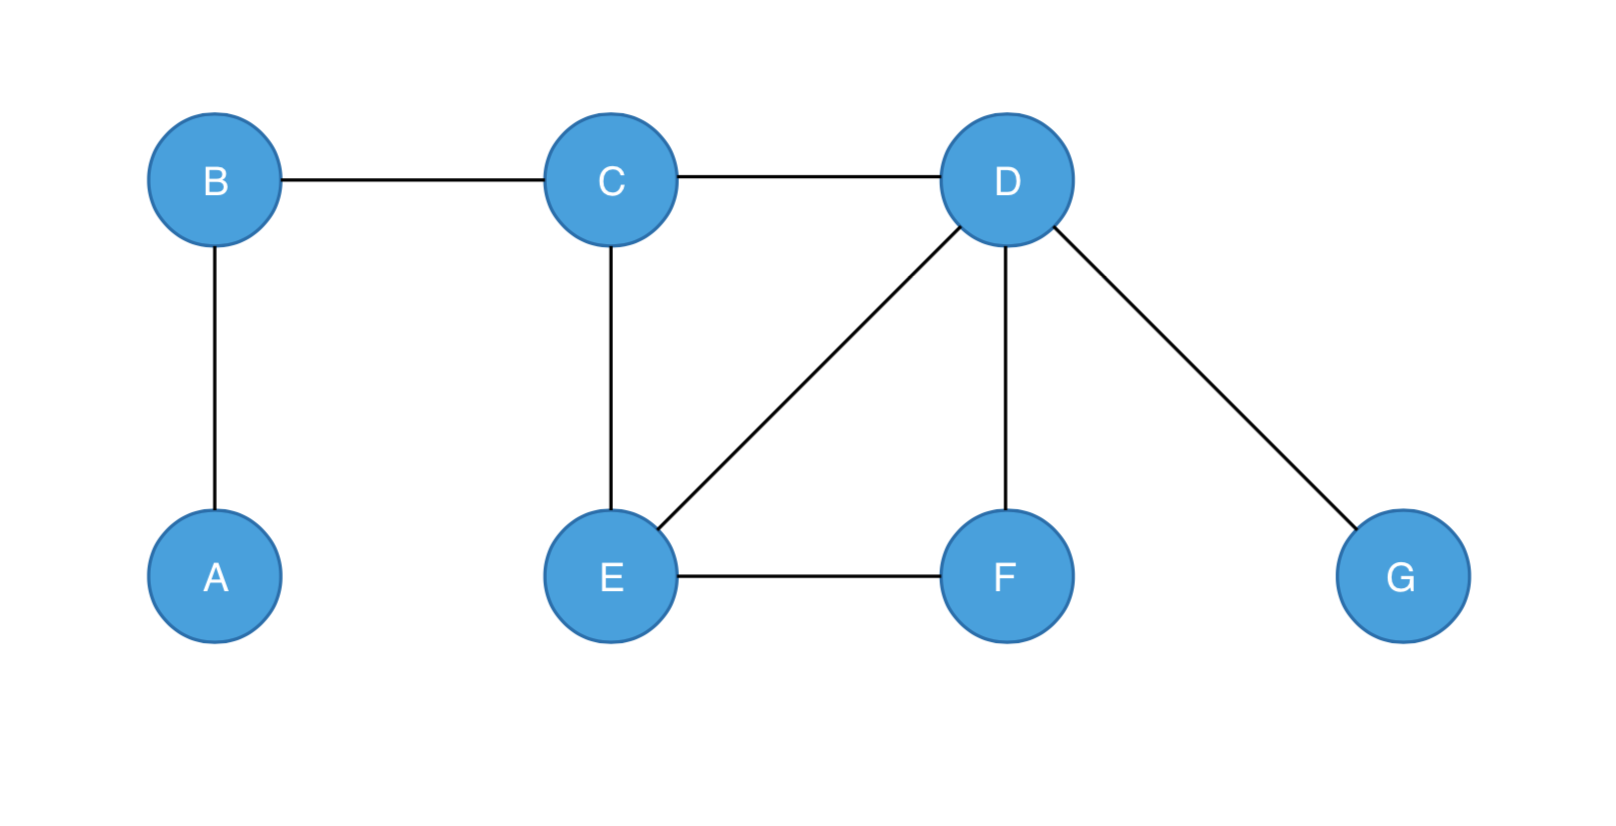
\includegraphics[height=4cm,width=9.5cm]{images/undirected.png}
	\caption{Undirected graph}
    \end{figure}
    \item \textbf{Directed graph}: When the set $E$ is represented as an ordered pair of vertices, it is called a directed graph or digraph. In a digraph, for some $x,y \in V(G)$, $(x,y) \neq (y,x)$.
    \begin{figure}[hbt!]
        \centering
	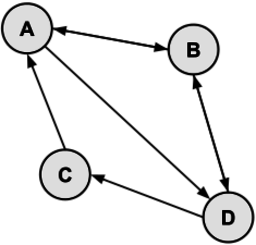
\includegraphics[height=4cm,width=7cm]{images/directed.png}
	\caption{Directed graph}
    \end{figure}
    \item \textbf{Multigraph}: If for any given vertices $x,y \in V(G)$, $\exists$ more than one edge $(x,y)$, then it is called a multigraph.
    \begin{figure}[hbt!]
        \centering
	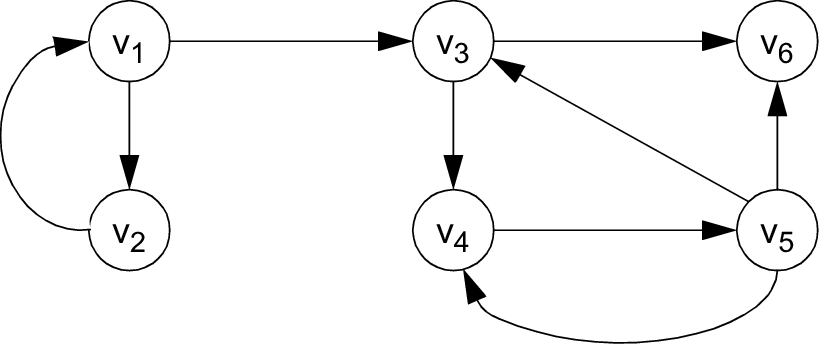
\includegraphics[height=4cm,width=9.5cm]{images/multi.png}
	\caption{Multigraph}
    \end{figure}
    \item \textbf{Pseudograph}: If for any given vertex, $x \in V(G)$, $\exists$ an edge $(x,x)$, that is, there is some edge $e$ that connects some vertex $x$ to itself.
    \begin{figure}[hbt!]
        \centering
	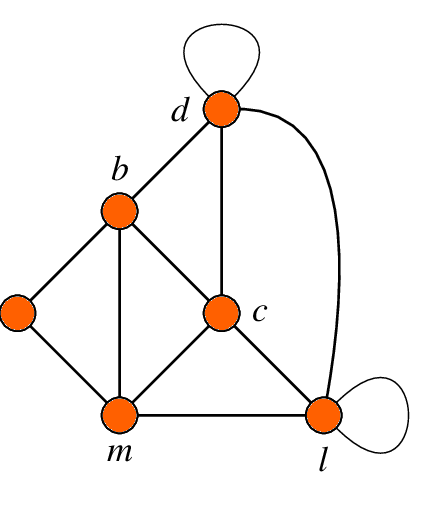
\includegraphics[height=3.82cm,width=7cm]{images/pseudo.png}
	\caption{Pseudograph}
    \end{figure}
    \item \textbf{Hypergraph}: If the edges of a graph are arbitrary subsets of vertices it is called hypergraph.
    \begin{figure}[hbt!]
        \centering
	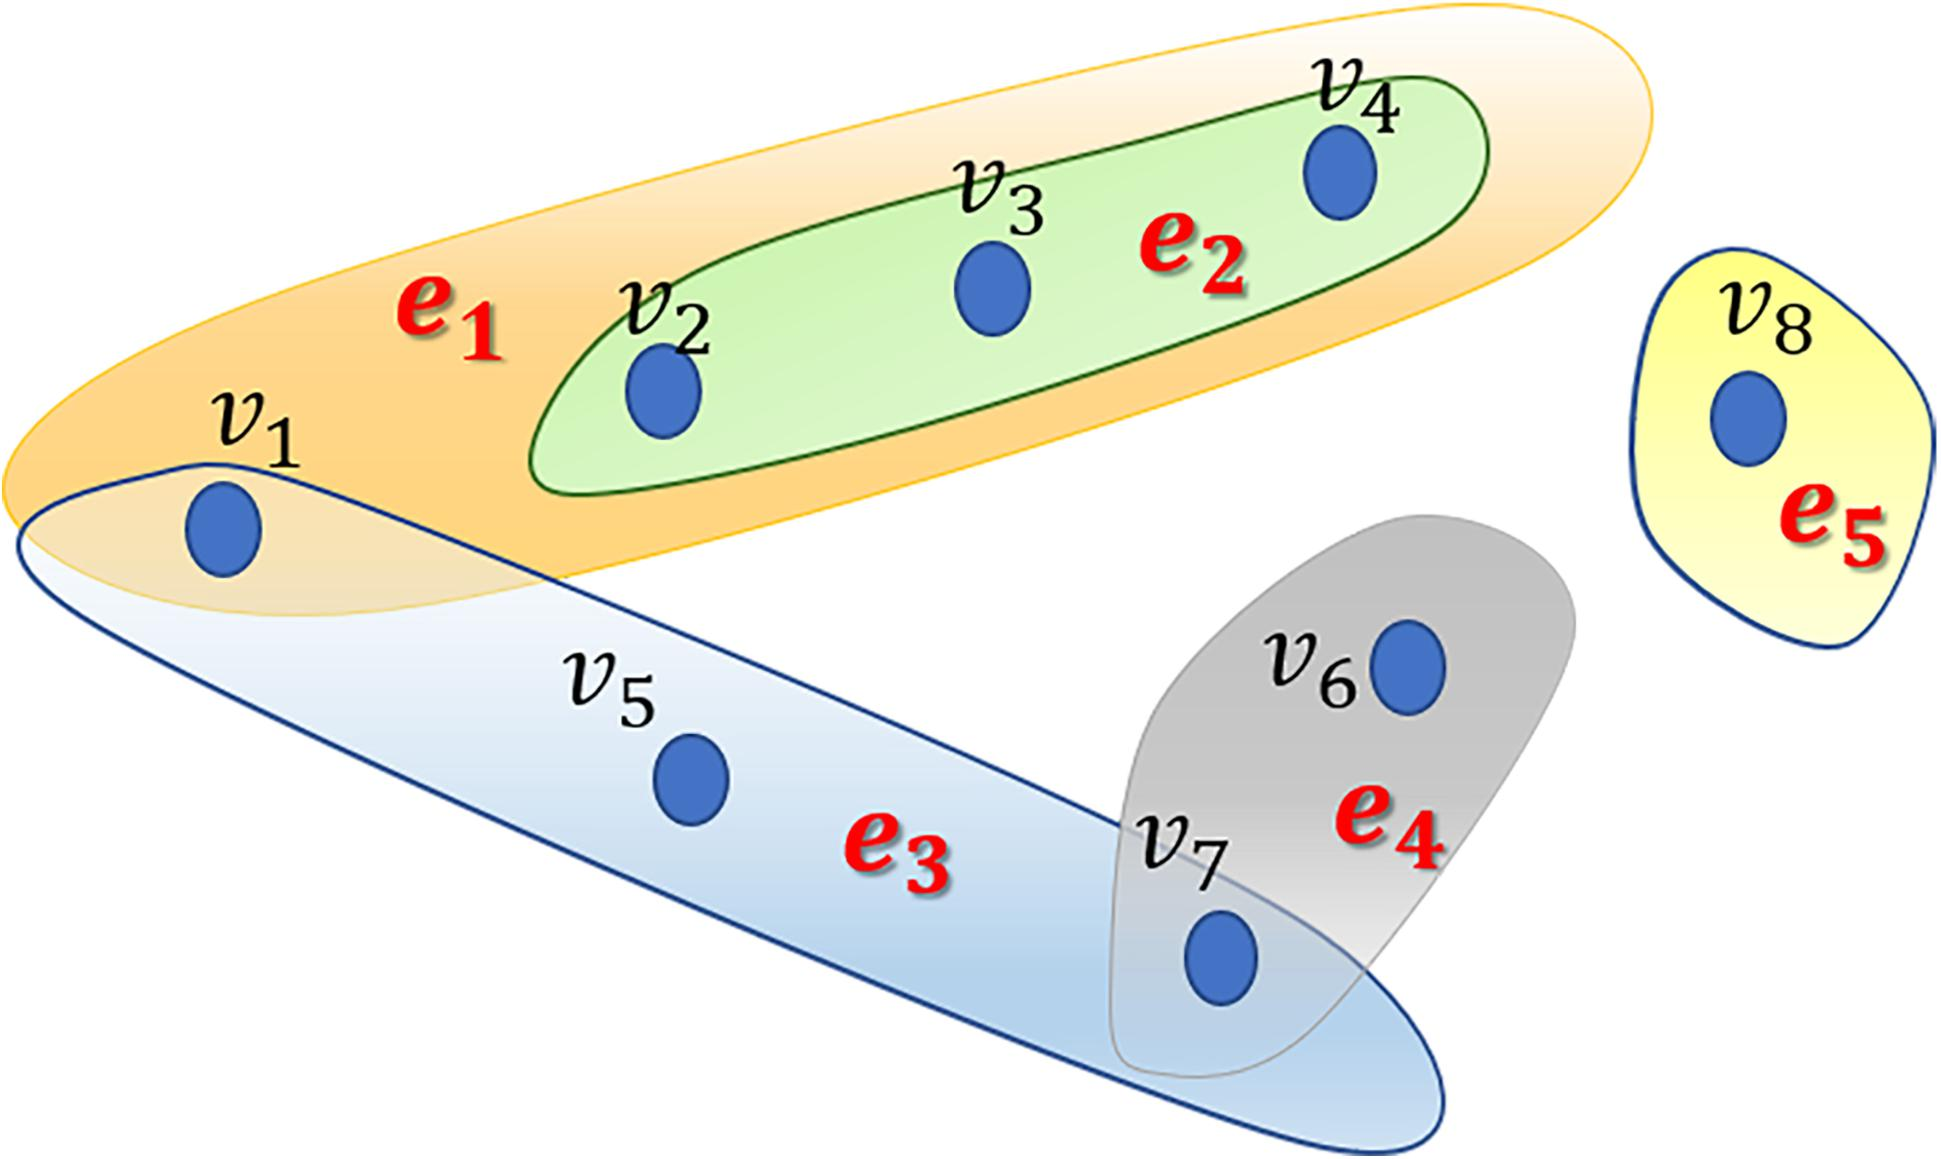
\includegraphics[height=4cm,width=9.5cm]{images/hyper.jpg}
	\caption{Hypergraph}
    \end{figure}
    \item \textbf{Infinite graph}: If the set $V$ or $E$ is infinite then it is called infinite graph.
\end{enumerate}

\chapter{Distance in Graphs}
\chapter{Trees}

A tree is a connected graph that contains no cycles. Graph-theoretic trees do not have cycles. A forest is a collection of one or more trees. A vertex of degree $1$ in a tree is called a leaf.\\
As in nature, graph-theoretic trees come in many shapes and sizes. They can be thin $(P_{10})$ or thick $(K_{1,1000})$, tall $(P_{1000})$ or short $(K_{1}$ and $K_{2})$. You can check out how these graphs look by looking them up on google.\\
There are some interesting names that can be assigned to certain graphs. Such as, $K_{1}$ is called a stump and $K_{2}$ is called a twig. Similarly, any $K_{1,3}$ graph is called a claw. There are more graphs, which have been assigned such interesting names, and the list is just a web search away from you.
\begin{thm}
    A tree $T$ of order $n$ has $(n-1)$ edges. 
\end{thm}
\begin{proof}
    We use induction to prove this theorem.\\
    Base Case: For $n=1$ the only tree is the stump $(K_{1})$, and it of course has $0$ edges.\\
    Induction Hypothesis:  Assume that the result is true for all trees of order less than $k$.\\
    Inductive Step: Let, $T$ be a tree of order $k$. Choose some edge of $T$ and call it $e$. Since $T$ is a tree, it must be that $T-e$ is disconnected with two connected components that are trees themselves. Say that these two components of $T-e$ are $T_{1}$ and $T_{2}$, with orders $k_{1}$ and $k_{2}$, respectively. Thus, $k_{1}$ and $k_{2}$ are less than $n$ and $k_{1} + k_{2} = k$.\\
    Since $k_{1} < k$, the theorem is true for $T_{1}$. Thus $T_{1}$ has $k_{1}-1$ edges. Similarly, $T_{2}$ has $k_{2}-1$ edges. Now, since $E(T)$ is the disjoint union of $E(T1)$, $E(T2)$, and $\{e\}$, we have $|E(T)|=(k_{1}-1) + (k_{2}-1) + 1 = k_{1} + k_{2} - 1 = k-1$.\\
    Hence, a tree $T$ of order $n$ has (n-1) edges.
\end{proof}

The next two theorems can be trivially proved by using the idea of the preceding theorem and so are left as an exercise for the reader.

\begin{thm}
    If $F$ is a forest of order $n$ containing $k$ connected components, then $F$ has $(n-k)$ edges.
\end{thm}

\begin{thm}
    A graph of order $n$ is a tree iff it is connected and contains $(n-1)$ edges.
\end{thm}

\begin{thm}
    If $T$ is a tree of order $n \ge 2$, then $T$ has atleast two leaves.
\end{thm}
\begin{proof}
    Readers van use theorem 1.0.5 and theorem 3.0.3 to prove this.
\end{proof}

\begin{thm}
    In any tree, the center is either a single vertex or a pair of adjacent vertices.
\end{thm}
\begin{proof}
Given a tree $T$, we form a sequence of trees as follows. Let $T_0 = T$. Let, $T_1$ be the graph obtained from $T_0$ by deleting all of its leaves. Note here that $T_1$ is also a tree. Let, $T_2$ be the tree obtained from $T_1$ by deleting all of the leaves of $T_1$. In general, for as long as it is possible, let $T_j$ be the tree obtained by deleting all of the leaves of $T_{j-1}$. Since $T$ is finite, there must be an integer $r$ such that $T_r$ is either $K_1$ or $K_2$.\\
Consider now a consecutive pair $T_i$, $T_{i+1}$ of trees from the sequence $T=T_0, T_1,..., T_r$. Let, $v$ be a non-leaf of $T_i$. In $T_i$, the vertices that are at the greatest distance from $v$ are leaves of $T_i$. This means that the eccentricity of $v$ in $T_{i+1}$ is one less than the eccentricity of $v$ in $T_i$. Since this is true for all non-leaves of $T_i$, it must be that the center of $T_{i+1}$ is exactly the same as the center of $T_i$.\\
Therefore, the center of $T_r$ is the center of $T_{r-1}$, which is the center of $T_{r-2}$,..., which is the center of $T_0=T$. Since, $T_r$ is either $K_1$ or $K_2$, the proof is complete.
\end{proof}

We will now add consider trees as subgraphs of graphs, that may or may not be trees.

\begin{thm}
Let $T$ be a tree with $k$ edges. If $G$ is a graph whose minimum degree satisfies $\delta(G) \ge k$, then $G$ contains $T$ as a subgraph. Alternatively, $G$ contains every tree of order at most $\delta(G)+1$ as a subgraph.
\end{thm}
\begin{proof}
We induct on $k$. If $k=0$, then $T=K_{1}$, and it is clear that $K_{1}$ is a subgraph of any graph. Further, if $k=1$, then $T=K_{2}$, and $K_{2}$ is a subgraph of any graph whose minimum degree is $1$. Assume that the result is true for all trees with $k-1$ edges $(k \ge 2)$, and consider a tree $T$ with exactly $k$ edges. We know that $T$ contains at least two leaves. Let, $v$ be one of them, and let, $w$ be the vertex that is adjacent to $v$. Consider the graph $T-v$. Since $T-v$ has $k-1$ edges, the induction hypothesis applies, so $T-v$ is a subgraph of $G$.\\
We can think of $T-v$ as actually sitting inside of $G$. Now, since $G$ contains at least $k+1$ vertices and $T-v$ contains $k$ vertices, there exist vertices of $G$ that are not a part of the subgraph $T-v$. Further, since the degree in $G$ of $w$ is at least $k$, there must be a vertex $u$ not in $T-v$ that is adjacent to $w$. The subgraph $T-v$ together with $u$ forms the tree $T$ as a subgraph of $G$.
\end{proof}

\begin{defn}
    Given a graph $G$, and a subgraph $T$, we say that $T$ is a spanning tree of $G$, if $T$ is a tree that contains every vertex of $G$.
\end{defn}

We end this chapter, by stating the famous Cayley's tree formula. We will not be including any proof for the theorem to keep things simple. However, the theorem has multiple interesting proofs. You can read them up from \say{Proofs from THE BOOK}.

\begin{thm}[Cayley's Tree formula]
    There are $n^{n-2}$ distinct labeled trees of order $n$.
\end{thm}

%The next parts of this chapter are not required for the Random Graphs WRP.
\documentclass[../basic_graph_theory.tex]{subfiles}

\begin{document}
\chapter{Paths, Trails, Cycles, and Circuits}
\setcounter{chapter}{4} %Set chapter counter
\setcounter{section}{0}
\setcounter{equation}{0}
\setcounter{figure}{0}

We start off this chapter by including some definitions. It would help you all to recall the definitions of paths, walks, and trails.

\begin{Def}{Cycle}{}
    A path which ends in the starting vertex is called a closed path or cycle.
\end{Def}
\begin{Def}{Circuit}{}
    A trail which ends in the starting vertex is called a closed trail or circuit.
\end{Def}
\begin{Def}{Eulerin trail}{}
    A trail in a graph $G$ that includes every edge of $G$ is called an Eulerian trail.
\end{Def}
\begin{Def}{Eulerian circuit}{}
    A circuit in a graph $G$ that includes every edge of $G$ is called an Eulerian circuit.
\end{Def}
\begin{Def}{Eulerian graph}{}
    A graph is said to be Eulerian if it has an Eulerian circuit.
\end{Def}
\begin{Def}{Hamiltonian path}{}
    If a path $P$ spans the vertices of $G$, then it is called a Hamiltonian path.
\end{Def}
\begin{Def}{Hamiltonian cycle}{}
    If a cycle $C$ spans the evrtices of $G$, then it is called a Hamiltonian cycle.
\end{Def}
\begin{Def}{Hamiltonian graph}{}
    A graph is said to be Hamiltonian if it has a Hamiltonian cycle.
\end{Def}

\begin{Thm}{}{}
    For a connected graph $G$, TFAE (the following are equivalent) :
    \begin{enumerate}
        \item[(i)] $G$ is Eulerian.
        \item[(ii)] Every vertex of $G$ has even degree.
        \item[(iii)] The edges of $G$ can be partitioned into edge-disjoint cycles.
    \end{enumerate}
\end{Thm}
The proof of this theorem is intuitive and are left as an exercise for the reader. It will be nice if you try to prove part (iii) and you can send your proofs on the group.
\begin{cor}
    The connected graph $G$ contains an Eulerian trail iff there are at most $2$ vertices of odd degree.
\end{cor}

Now, we state two very important theorems that will be used both in our Random Graphs WRP as well as in many graph theoretic problems that you may encounter in future.

\begin{Thm}{Dirac's theorem}{}
    Let, $G$ be a graph of order $n \ge 3$. If $\delta(G) \ge \frac{n}{2}$, then $G$ is Hamiltonian.
\end{Thm}
\begin{proof}
    Suppose $G$ is a counterexample to the theorem and $G$ be such a graph with maximal number of edges i.e., addition of an edge to $G$ creates a cycle.  Let $v \nsim w$ and hence $G \cup (v,w)$ will contain a Hamilton cycle $v = v_1v_2\ldots v_n=w,v$. Thus $v_1v_2\ldots v_n$ is a simple path. Define sets $S_v \coloneqq \{ i : v \sim v_{i+1} \}$ and $S_w \coloneqq \{ i : w \sim v_i\}$. Since $\delta(G) \geq n/2$, $|S_v|, |S_w| \geq n/2$ and further $S_v, S_w \subset \{1,\ldots,n-1\}$. Hence $S_v \cap S_w \neq \emptyset$ and assume that $i_0 \in S_v \cap S_w$. Then $v = v_1v_2\ldots v_{i_0}w=v_nv_{n-1}\ldots v_{i_0+1}v_1=v$ is a Hamiltonian circuit in $G$, contradicting our assumption.
\end{proof}

\begin{Thm}{Ore's theorem}{}
    Let, $G$ be a graph of order $n \ge 3$. If $deg(x)+deg(y) \ge n$, then $\forall$ pairs of non-adjacent vertices $x,y$, then $G$ is Hamiltonian.
\end{Thm}

The proof of this theorem is left as an exercise to the reader. You can make use of Dirac's theorem as well as the approach used in it's proof to prove Ore's theorem. We encourage you to share your proof in the group.\\
Next, we define some very useful terminologies that will be of essence.\\

\begin{Def}{Independent sets and covers}{} \index{independent sets} \index{cover}
    An {\em independent set of vertices} is $S \subset V$ such that no two vertices in $S$ are adjacent. An {\em independent set of edges} is $E' \subset E$ such that no two edges in $E'$ share a common end vertex. A subset of vertices $S \subset V$ is a {\em vertex cover} if every edge in $G$ is incident to at least one vertex in $S$. An {\em edge cover} is a set of edges $E' \subset E$ such that every vertex is contained in at least one edge in $E'$.
\end{Def}
\begin{Def}{Independence number and cover number}{}
    %
    \begin{eqnarray*}
        \alpha(G) & = & \max \{|S| : S \, \mbox{independent vertex set} \}. \\
        \alpha'(G) & = & \max \{|M| : M \, \mbox{independent edge set} \}. \\
        \beta(G) & = & \min \{|S| : S \, \mbox{vertex cover} \}.  \\
        \beta'(G) & = & \min \{|E'| : E' \, \mbox{edge cover} \}.
    \end{eqnarray*}
\end{Def}

Now we will state a very interesting theorem which relates the Hamiltonicity of a graph with it's connectivity and independence number.

\begin{Thm}{}{}
    Let, $G$ be a connected graph of order $n \ge 3$ with vertex connectivity $\kappa(G)$ and independence number $\alpha(G)$. If $\kappa(G) \ge \alpha(G)$, then G is Hamiltonian.
\end{Thm}
You can skip the proof of this theorem if you want, as the proof would not be a crucial part of our WRP.
\begin{proof}
    If $G$ is as described, then $\kappa(G) \ge 2$, as if $\kappa(G)=1$, then $\alpha(G)=1$ and thus $G$ is either $K_1$ or $K_2$, contradicting the fact that $n \ge 3$.\\
    Let $C$ be a longest cycle in $G$. Suppose that $C$ is not a Hamiltonian cycle, and let $v$ be a vertex of $G$ that is not on $C$. Let, $H$ be the connected component of $G-V(C)$ containing vertex $v$.\\
    $V(C)=\{c_1,c_2,\dots,c_r\}$\\
    The vertex of $H$ adjacent to $c_i$ is denoted by $h_i$. The vertex which is the immediate clockwise successor of $c_i$ is denoted by $d_i$.\\
    Following these, we can make some observations:\\
    \begin{enumerate}
        \item[(i)] It must be that $r \ge \kappa(G)$. If the vertices $V(C)$ were removed from $G$, then $H$ would be disconnected from the rest of the graph. Since $\kappa(G)$ is the size of the smallest cut set, it follows that $r \ge \kappa(G) \ge 2$.
        \item[(ii)] No two of the vertices in the set $V(C)$ are consecutive vertices on $C$. To see this, suppose that there is some $i$ such that $c_i$ and $c_{i+1}$ are consecutive vertices on $C$. Let, $P$ be a path from $h_i$ to $h_{i+1}$ in $H$, and consider the cycle formed by replacing the edge $c_ic_{i+1}$ on $C$ with the path $c_i, [h_i, h_{i+1}]_{P} , c_{i+1}$. This cycle is longer than our maximal cycle $C$, a contradiction. This observation implies that the sets ${c_1, c_2,\dots,c_r}$ and ${d_1, d_2,\dots,d_r}$ are disjoint.
        \item[(iii)] For each $i (1 \le i \le r)$, $d_i$ is not adjacent to $v$. To see this, suppose $d_{i}v \in E(G)$ for some $i$, and let $Q$ be a path from $h_i$ to $v$ in $H$. In this case, the cycle formed by replacing the edge $c_{i}d_{i}$ on $C$ with the path $c_{i}, [h_{i}, v]_{Q}, d_{i}$ is longer than $C$, again a contradiction.
    \end{enumerate}
    Now, let $S = {v,d_1, d_2,...,d_r}$. The first observation above implies that $|S| \ge \kappa(G)+1 > \alpha(G)$. This means that some pair of vertices in $S$ must be adjacent. Our third observation implies that $d_i$ must be adjacent to $d_j$ for some $i<j$. If $R$ is a path from $h_i$ to $h_j$ in $H$, then the cycle $c_i, [h_i, h_j]_{R}, [c_j , d_i]_{C^-} , [dj , ci]_{C^+}$ is a longer cycle than $C$. Our assumption that $C$ was not a Hamiltonian cycle has led to a contradiction and thus, $C$ is indeed a Hamiltonian cycle.
\end{proof}

Next, we introduce the idea of forbidden subgraphs. The absence of any particular forbidden subgraph $H$ in a graph $G$, gives $G$ some ``nice'' properties. This concept of forbidden subgraphs will be very crucial in understanding and checking for planarity of graphs. Here, we will relate forbidden subgraphs to Hamiltonicity. For the next two theorems, you may skip the proofs if you wish.

\begin{Thm}{}{}
    If $G$ is a $2$-connected, $\{K_{1,3}, Z_{1}\}$-free graph, then $G$ is Hamiltonian
\end{Thm}
\begin{proof}
    Suppose $G$ is $2$-connected and ${K_{1,3}, Z_1}$-free, and let $C$ be a longest cycle in $G$. If $C$ is not a Hamiltonian cycle, then there must exist a vertex $v$, not on $C$, which is adjacent to a vertex, say $w$, on $C$. Let $a$ and $b$ be the immediate predecessor and successor of $w$ on $C$.\\
    A longer cycle would exist if either $a$ or $b$ were adjacent to $v$, and so it must be that both $a$ and $b$ are nonadjacent to $v$. Now, if $a$ is not adjacent to $b$, then the subgraph induced by the vertices ${w,v,a,b}$ is $K_{1,3}$, and we know that $G$ is $K_{1,3}$-free. So it must be that $ab \in E(G)$. But if this is the case, then the subgraph induced by ${w,v,a,b}$ is $Z_1$, a contradiction. Therefore, it must be that $C$ is a Hamiltonian cycle.
\end{proof}

\begin{Thm}{}{}
    \label{ref:1}
    Let, $G$ be a $\{K_{1,3}, N\}$-free graph. Then:\\
    \begin{enumerate}
        \item If $G$ is connected, then $G$ is traceable.
        \item If $G$ is $2$-connected, then $G$ is Hamiltonian.
    \end{enumerate}
\end{Thm}

The proof of the second part follows directly from theorem \ref{ref:1}. The proof of the first part is also simple and the only obstacle that may arise is understanding what we mean by traceable. A traceable graph refers to a graph that has a Hamiltonian path.
\begin{figure}[htbp]
    \tikzset{every picture/.style={line width=0.75pt}}
    \begin{center}
        \begin{tikzpicture}[x=0.65pt,y=0.65pt,yscale=-0.5,xscale=0.5]
            \draw  (326,92) -- (399,202.41) ;
            \draw  (326,92) -- (254,202.41) ;
            \draw  (254,202.41) -- (399,202.41) ;
            \draw  (327,18.41) -- (326,92) ;
            \draw  (474,249.41) -- (399,202.41) ;
            \draw  (182,246.41) -- (254,202.41) ;
        \end{tikzpicture}
    \end{center}
    \caption{This graph is represented by \textbf{N}}
\end{figure}

\end{document}
\documentclass[../basic_graph_theory.tex]{subfiles}

\begin{document}
\chapter{Matchings}
\setcounter{chapter}{5} %Set chapter counter
\setcounter{section}{0}
\setcounter{equation}{0}
\setcounter{figure}{0}

\section{Matchings}

\begin{Def}{Matching}{matching} \index{Matching}\index{Perfect Matching}
    A subset $M$ of edges is said to be \textbf{matching} if no two edges are incident on any vertex or equivalently, every vertex is contained in at most one edge. A {complete matching} $M$ on a subset $S \subset V$ is a matching that contains all the vertices in $S$. A \textbf{perfect matching} is a complete matching on $G$.
\end{Def}

Alternatively one can consider a matching of a graph $M$ as a subgraph of $G$ such that $d_M(v) = 1$ for all $v \in V(M)$. A matching is perfect if $M$ is spanning. A vertex $v$ is said to be {\em saturated} if $v \in M$ and else {\em unsaturated}. For a subset $S \subset V$, $N(S) = \bigcup_{v \in S}N(v).$

\begin{Thm}{Hall's marriage theorem}{} \index{Hall's marriage theorem}
    Let $G$ be a bi-partite graph with the two vertex sets being $V_1,V_2$.  Then there exists a complete matching on $V_1$ iff $|N(S)| \geq |S|$ for all $S \subset V_1$.
\end{Thm}

\begin{proof}
    Let $|V_1| = k$ and our proof will be by induction on $k$. If $k = 1$, the proof is trivial. Let $G = V_1 \cup V_2$ be such that the result holds for any graph with strictly smaller $V_1$.
    
    Suppose that $|N(S)| \geq |S| + 1$ for all $S \subsetneq V_1$. Then choose $(v,w) \in E \cap V_1 \times V_2$ and consider the induced subgraph $G' := \langle V - \{v,w\} \rangle$. Since we have removed only $w$ from $V_2$ and that $|N(S)| \geq |S| + 1$ for all $S \subsetneq V_1$, we get that $|N(S')| \geq |S'|$ for all $S' \subset V_1 - \{v\}$. Thus there is a complete matching $M$ on $V_1 - \{v\}$ in $G'$ by induction hypothesis and $M \cup (v,w)$ is a complete matching on $V_1$ in $G$ as desired.

    If the above is not true i.e., there exists $A \subset V_1$ such that $N(A) = B$ and $|A| = |B|$. Then, by induction hypothesis, there is a complete matching $M_0$ on $A$ in the induced subgraph $\langle A \cup B \rangle$. Trivially,  Hall's condition holds i.e., for all $S \subset A$,  $|N(S) \cap B| =  |N(S)| \geq |S|$. Let $G' := G - \angle  A \cup B \rangle$.  Let $S \subset V_1 - A$.  Suppose if $|N'(S)| < |S|$ where $N'(S) = N(S) \cap (V_2 - B)$.  Then,  we have that $N(S \cup A) = N'(S) \cup B$ and hence $|N(S \cup A)| \leq |N'(S)| + |B| < |S| + |A|$,  a contradiction.  Hence, $G'$ also satisfies Hall's condition and again by induction hypothesis $G'$ has a complete matching $M'$ on $V_1 -A$. Thus, we have a complete matching $M := M_0 \cup M'$ on $V_1$ in $G$.
\end{proof}

\begin{prop}
    Let $d \geq 1$. Let $G$ be a bipartite graph on $V_1 \sqcup V_2$ such that $|N(S)| \geq |S| - d$ for all $S \subset V_1$. Then $G$ has a matching with at least $|V_1| - d$ independent edges.
\end{prop}

\begin{proof}
    Set $V'_2 := V_2 \cup [d]$. Define $G'$ with vertex set as $V_1 \sqcup V'_2$ and edge set as $E(G) \cup (V_1 \times [d])$. Then, it is easy to see that Hall's condition is true on $G'$ and hence there is a complete matching $M$ of $V_1$ in $G'$. Now, if we remove the edes in $M$ incident on $[d]$, we get a matching with at least $|V_1| - d$ edges as required.
\end{proof}

\begin{Def}{}{}[Factor of a graph \index{factor}]
    Given a graph $G$,  a factor of $G$ is a spanning subgraph.  Equivalently,  a subgraph $H$ is said to be a factor (of $G$) if $V(H) = V(G)$. An $r$-factor is a factor that is $r$-regular.
\end{Def}

Thus, $1$-factors are nothing but perfect matchings.

\begin{Thm}{Petersen, 1891}{}
    Every regular graph of positive even degree has a $2$-factor.
\end{Thm}
\begin{proof}
    Easy exercise.
\end{proof}

A matching $M$ is said to be {\em maximal} if there is no matching $M'$ such that $M \subsetneq M'$.  A matching $M$ is said to be {\em a maximum matching} if $\alpha'(G) = |M|$.

Now recall the definitions of $\alpha(G), \beta(G), \alpha'(G), \beta'(G)$. If $M$ is a maximum matching, then to cover each edge we need distinct vertices and hence the vertex cover should have size at least $|M|$.  Furthermore,  given a maximum matching $M$,   $V(M)$ gives a vertex cover.   For if there is an edge $e$ not covered by $V(M)$ then $M+e$ is a larger matching than $M$.  These observations yield the first inequality below.
\[
    \alpha'(G) \leq  \beta(G) \leq 2 \alpha'(G) \text{ and } \alpha(G) \leq \beta'(G)
\]
As for the second inequality, observe that to cover vertices of an independent set, we need distinct edges.

\begin{lem}
    Let $G$ be a graph. $S \subset V$ is an independent set iff $S^c$ is a vertex cover. As a corollary, we get $\alpha(G) + \beta(G) = n = |V|.$
\end{lem}
\begin{Thm}{Konig-Egervary theorem}{} \index{Konig-Egervary theorem}
    For a bi-partite graph, $\alpha'(G) = \beta(G)$.
\end{Thm}
\begin{proof}
    We will show that for a minimum vertex cover $Q$, there exists a matching of size at least $|Q|$. Partition $Q$ into $A := Q \cap V_1$ and $B := Q \cap V_2$. Let $H$ and $H'$ be induced subgraphs on $A \sqcup (V_2 - B)$ and $(V_1 - A) \sqcup B$ respectively. If we show that there is a complete matching on $A$ in $H$ and a complete matching on $B$ in $H'$, we have a matching of size at least $|A| + |B|$ ($= |Q|$) in $G$.  Also, note that it suffices to show that there is a complete matching on $A$ in $H$ because we can reverse the roles of $A$ and $B$ apply the same argument to $B$ as well. \\
    Since $A \cup B$ is a vertex cover, there cannot be an edge between $V_1 - A$ and $V_2 - B$. Suppose for some $S \subset A$, we have that $|N_H(S)| < |S|$. Since $N_H(S)$ covers all edges from $S$ that are not incident on $B$, $Q' := Q - S + N_H(S)$ is also a vertex cover. By choice of $S$, $Q'$ is a smaller vertex cover than $Q$ contradicting that $Q$ is minimum.  Hence, we have that Hall's condition holds true for $A$ in $H$. And by the arguments in the previous paragraph, the proof is complete.
\end{proof}
\begin{Thm}{Gallai, 1959}{} \index{Gallai theorem}
    If $G$ is a graph without isolated vertices, then $\alpha'(G) + \beta'(G) = n = |V|.$
\end{Thm}

\begin{proof}
    Suppose $M$ is a maximum matching. Then $S = V - V(M)$ is also an independent set. If there are edges between vertices of $S$, then such edges can be added to $M$ and one can obtain a larger matching. Hence there are no edges between vertices of $S$ and hence it is a independent set. Construct a edge cover as follows : Add all edges in $M$ to $Q$ and for each $v \in S$, add one of its adjacent edges to $Q$.  Since there are no isolated vertices,  $v$ has atleast one adjacent edge.  Thus $|Q| = |M| + |S|$ and since $V(M) \sqcup S = V$, we can derive that
    \[
        \alpha'(G) + \beta'(G) \leq |M| + |Q| = 2|M| + |S| = n
    \]
    Let $Q$ be a minimum edge cover. Then $Q$ cannot contain a path of length more than $2$. Else, by removing the middle edge in a path of length at least 3, we can obtain a smaller edge cover. By the previous exercise, $Q$ is a graph consisting of star components. If $C_1,\ldots,C_k$ are the components of $Q$, then $V(C_1) \cup \ldots \cup V(C_k) = V$ and $E(C_1) \cup \ldots \cup E(C_k) = Q$. Now choose a matching $M = \{e_1,\ldots,e_k\}$ by selecting one edge from every component $C_1,\ldots,C_k$.  Since $C_i$'s are disjoint, $M$ is a matching. Thus, using the fact that each $Q$ is a forest with $k$ components, we can derive that
    \[
        \alpha'(G) + \beta'(G)  \geq |M| + |Q| = k + |E(Q)| = n
    \]
\end{proof}

As a corollary, we get K\"{o}nig's result : if $G$ is bi-partite graph without isolated vertices, $\alpha(G) = \beta'(G)$.

\section{Augmenting path}

\begin{Def}{Augmenting path}{aug:path}\index{augmenting path}
    Given a matching $M$, a $M$-alternating path $P$ is a path such that its edges alternate between $M$ and $M^c$.  A $M$-augmenting path is a $M$-alternating path whose end-vertices do not belong to $M$.
\end{Def}

\begin{Thm}{Berge, 1957}{}\index{Berge theorem}
    A matching $M$ in a graph is a maximum matching in $G$ iff $G$ has no $M$-augmenting path.
\end{Thm}

\begin{proof}
    Suppose there is an $M$-augmenting path $P$. Let $P = v_0v_1\ldots v_k$. Since $P$ is $M$-augmenting, $(v_0,v_1),(v_2,v_3),\ldots,(v_{k-1},v_k) \notin M$ and $(v_1,v_2), (v_3,v_4),\ldots,(v_{k-2},v_{k-1}) \in M$.  Now, observe that $M' = M - P \cup \{ (v_0,v_1),(v_2,v_3),\ldots,(v_{k-1},v_k) \}$ is a larger matching than $M$. Hence if $M$ is a maximum matching, there is no $M$-augmenting path.
    \begin{figure}[htbp]
        \centering
        \tikzset{every picture/.style={line width=0.75pt}} % set default line width to 0.75pt
        \begin{tikzpicture}[x=0.75pt,y=0.75pt,yscale=-1,xscale=1]
            Straight Lines [id:da2542280834688819]
            \draw [color={rgb, 255:red, 74; green, 144; blue, 226 }  ,draw opacity=1 ]   (152,169) -- (226.8,125) ;
            %Straight Lines [id:da1803665588330392] 
            \draw [color={rgb, 255:red, 208; green, 2; blue, 27 }  ,draw opacity=1 ]   (226.8,125) -- (298.8,171) ;
            %Straight Lines [id:da4946128828587528] 
            \draw [color={rgb, 255:red, 74; green, 144; blue, 226 }  ,draw opacity=1 ]   (298.8,171) -- (373.6,127) ;
            %Straight Lines [id:da6019832013239967] 
            \draw [color={rgb, 255:red, 208; green, 2; blue, 27 }  ,draw opacity=1 ]   (373.6,127) -- (445.6,173) ;
            %Straight Lines [id:da9998485691080525] 
            \draw [color={rgb, 255:red, 74; green, 144; blue, 226 }  ,draw opacity=1 ]   (445.6,173) -- (520.4,129) ;
        \end{tikzpicture}
        \caption{Red is a maximal matching and Blue is a maximum matching}
        \label{fig:matching paths}
    \end{figure}
    Suppose $M'$ is a larger matching than $M$. We shall construct an $M$-augmenting path and prove the theorem by contraposition. Let $F = M \triangle M'$. We know by the above exercise that the components of $F$ are paths or even cycles. Since $|M'| > |M|$, there must be a component of $F$ such that $M'$ has more edges in that component than $M'$. If a component in $F$ is an even cycle, it consists of same number of edges from $M$ and $M'$. Thus, the component for which $M'$ has more edges must be a path, say $P = v_0\ldots,v_k$. Since $P \subset F$, we have that $P$ has to be an $M$-alternating path i.e., $(v_0,v_1) \in M', (v_1,v_2) \in M, \ldots$ or $(v_0,v_1) \in M, (v_1,v_2) \in M', \ldots$. Since $m' := |M' \cap P| > |M \cap P| = m$ and that $P$ is an $M$-alternating path,  we derive that $m' - m = 1$ and $k = 2m + 1$.  Further, this implies that $(v_0,v_1),(v_2,v_3),\ldots,(v_{k-1},v_k) \in M'$ and $(v_1,v_2), (v_3,v_4),\ldots,(v_{k-2},v_{k-1}) \in M$ i.e.,  $P$ is an $M$-alternating path.   If $v_0 \in V(M)$ then there exists $(w,v_0) \in M$ for some $w \neq v_1$.  Also $(w,v_0) \in M \setminus M' \subset F$ contradicting the assumption that $P$ is not a component.   So $v_0 \notin M$ and similarly $v_k \notin M$.   Thus,  we have that $P$ is an $M$-augmenting path as needed.
\end{proof}
Recall definition of graph factors.  For a graph $G$, let $o(G)$ denote the number of odd components of $G$. The next theorem that we will be stating has a long proof and you may skip it if you want.

\begin{Thm}{Tutte's 1-factor theorem}{}\index{Tutte's factor theorem}
    A graph has a $1$-factor iff $o(G-S) \leq |S|$ for all $S \subset V$.
\end{Thm}
\begin{proof}
    \textbf{\textit{To Be Added\dots}}
\end{proof}
We end this chapter by stating Menger's theorem. However, before diving into the theorem we need to look at some definitions.

\ssk

Let $G$ be a connected graph, and let $u$ and $v$ be vertices of $G$. If $S$ is a subset of vertices that does not include $u$ or $v$, and if the graph $G-S$ has $u$ and $v$ in different connected components, then we say that $S$ is a $u,v$-separating set.

\begin{Thm}{}{}
    Let $G$ be a graph and let $u$ and $v$ be vertices of $G$. The maximum number of internally disjoint paths from $u$ to $v$ equals the minimum number of vertices in a $u,v$-separating set.
\end{Thm}
You can skip the proof of this theorem if you wish.
\begin{proof}
    \textbf{\textit{To Be Added\dots}}
\end{proof}
\end{document}
\documentclass[../basic_graph_theory.tex]{subfiles}

\begin{document}
\chapter{Planarity}
\setcounter{chapter}{6} %Set chapter counter
\setcounter{section}{6}
\setcounter{equation}{6}
\setcounter{figure}{6}

A graph $G$ is said to be planar if it can be drawn in the plane in such a way that pairs of edges intersect only at vertices, if at all. If $G$ has no such representation, $G$ is called nonplanar. A drawing of a planar graph $G$ in the plane in which edges intersect only at vertices is called a planar representation (or a planar embedding) of $G$.\\

If three or more edges bound a portion of a graph then we call it a region. In figure \ref{ref:regions}, $R_1, R_2, \dots, R_7$ are regions in the graph. An edge $e$ bounds a region $R$, if it comes in contact with $R$. We denote the bound degree of $R$ by $b(R)$ and define it as the number of edges that bound region $R$.

\begin{figure}[hbt!]
    \label{ref:regions}
    \centering
    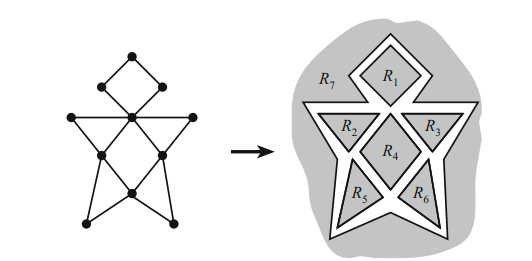
\includegraphics[height=4cm,width=9.5cm]{images/region.png}
    \caption{Representation of regions in a graph}
\end{figure}

Now, we are ready to state the famous Euler's formula.
\begin{thm}[Euler's formula]
    For a connected planar graph $G$ with $n$ vertices, $q$ edges, and $r$ regions, then $n-q+r=2$.
\end{thm}
\begin{proof}
    We induct on $q$, the number of edges. If $q = 0$, then $G$ must be $K_1$, a graph with $1$ vertex and $1$ region. The result holds in this case. Assume that the result is true for all connected planar graphs with fewer than $q$ edges, and assume that $G$ has $q$ edges.\\
    \em{Case 1.} Suppose $G$ is a tree. We know from our work with trees that $q = n-1$, and $r = 1$, since a planar representation of a tree has only one region. Thus, $n - q + r = n - (n - 1) + 1 = 2$, and the result holds.\\
    \em{Case 2.} Suppose $G$ is not a tree. Let $C$ be a cycle in $G$, let e be an edge of $C$, and consider the graph $G - e$. Compared to $G$, this graph has the same number of vertices, one edge fewer, and one region fewer, since removing e coalesces two regions in $G$ into one in $G - e$. Thus the induction hypothesis applies, and in $G - e$, $n - (q - 1) + (r - 1) = 2$, implying that $n - q + r = 2$.\\
    The result holds in both cases, and the induction is complete.
\end{proof}

Euler's formula helps us a lot in identifying non-planar graphs. We urge you to check using Euler's formula that $K_{3,3}$ and $K_5$ are non-planar. A more general general version of the Euler's formula has been stated below.

\begin{thm}
    For a planar graph $G$ with $n$ vertices, $q$ edges, and $r$ regions, then $n-q+r=1+\beta_{0}(G)$.
\end{thm}

\begin{thm}
    If $G$ is a planar graph with $n \ge 3$ vertices and $q$ edges, then $q \le 3n - 6$. Furthermore, if equality holds, then every region is bounded by three edges.
\end{thm}
\begin{proof}
    Let, us consider $C=\sum_{R}b(R)$.\\
    Since every edge of $G$ is shared by at most $2$ regions so, $C \le 2q$. Further as each region is bounded by atleast $3$ edges, so $C \ge 3r$. Thus,\\
    \begin{align*}
        &3r \le 2q\\
        \Longrightarrow &3(2+q-n) \le 2q\\
        \Longrightarrow &6+3q-3n \le 2q\\
        \Longrightarrow &q \le 3n-6\\
    \end{align*}
    If equality holds, then $3r = 2q$, and it must be that every region is bounded by three edges.
\end{proof}

\begin{thm}
    If $G$ is a planar graph, then $\delta(G) \le 5$.
\end{thm}
\begin{proof}
    Suppose $G$ has $n$ vertices and $q$ edges. If $n \le 6$, then the result is immediate, so we will suppose that $n > 6$. If we let $D$ be the sum of the degrees of the vertices of $G$, then we have:\\
    \begin{equation*}
        D = 2q \le 2(3n - 6) = 6n - 12
    \end{equation*}
    If each vertex had degree $6$ or more, then we would have $D \ge 6n$, which is impossible. Thus there must be some vertex with degree less than or equal to $5$.
\end{proof}

Now, we define what we mean by a subdivision as the concluding portion of this chapter will cover two theorems that are very important and will go a long way in helping us outright identify many graphs as non-planar.\\

\begin{defn}
    A subdivision of an edge $G$ is a substitution of a path for $e$.
\end{defn}
\begin{defn}
    We say that, $H$ is a subdivision of $G$ if $H$ can be obtained from $G$ by a finite sequence of subdivisions.
\end{defn}

Now that the idea of subdivisions has been introduced we can finally move on to the last two theorems for this chapter.
\begin{thm}
    A graph $G$ is planar iff every subdivision of $G$ is planar.
\end{thm}
The proof for this is very intuitive as so is left as an exercise for the reader.\\
Lastly, we end this chapter by stating and proving Kuratowski's theorem.\\
\begin{thm}
    A graph $G$ is planar iff it contains no subdivision of $K_{3,3}$ or $K_{5}$.
\end{thm}
We state this theorem without proof as the proof is not very easy. However, you acn check out the proof of Kuratowski's theorem online.

\end{document}
\chapter{Colorings}
\documentclass[../basic_graph_theory.tex]{subfiles}

\begin{document}
\chapter{Spectral Graph Theory}
\addcontentsline{toc}{chapter}{Spectral Graph Theory} %Set chapter title
\setcounter{chapter}{8} %Set chapter counter
\setcounter{section}{8}
\setcounter{equation}{8}
\setcounter{figure}{8}


\end{document}
\documentclass[../basic_graph_theory.tex]{subfiles}

\begin{document}
\chapter{Some Basic Exercises}
\setcounter{chapter}{9} %Set chapter counter
\label{chap:exercises}
\setcounter{section}{0}
\setcounter{equation}{0}
\setcounter{figure}{0}

\end{document}
\documentclass[../basic_graph_theory.tex]{subfiles}

\begin{document}
\chapter{***Challenge Problems***}
\addcontentsline{toc}{chapter}{***Challenge Problems***} %Set chapter title
\setcounter{chapter}{3} %Set chapter counter
\setcounter{section}{3}
\setcounter{equation}{3}
\setcounter{figure}{3}


\end{document}
\end{document}
